%! Author = gramic
%! Date = 08.04.24

% Preamble
\subsubsection{yugabyteDB}
\begin{flushleft}
    \paragraph{1. Testing}
    Beim ersten Testing hat sich mutmasslich das Storage system von \gls{local-path-provisioner} einen Fehler erzeugt.\\
    Es wurde ein Zeitsystem-Fehler geworfen, allerdings gab \gls{chrony} keine Synchronisationsprobleme zurück.\\
    \begin{figure}[H]
        \centering
        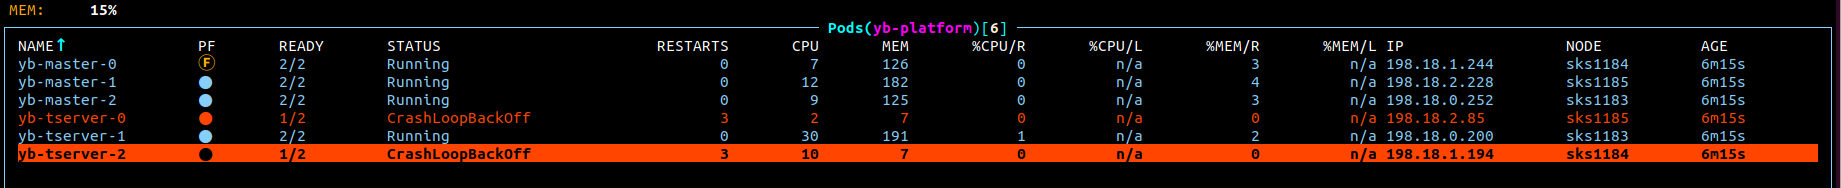
\includegraphics[width=0.8\linewidth]{source/implementation/evaluation/evaluation_tests/storage_errors/k8s_crashloopback}
        \caption{yugabyteDB - Evaluation-Testing - CrashLoopBackOff}
        \label{fig:k8s_crashloopback}
    \end{figure}
\end{flushleft}
\begin{flushleft}
    Als Ursache wurde das Storage system ermittelt, weil weder das neuerstellen des yugabyteDB-Namespace noch die  neuinstallation aller Pods abhilfe schaffte.\\
    Erst als \gls{local-path-provisioner} komplett gesäubert und neu aufgesetzt wurde, konnte der Test sauber neu aufgebaut werden.
\end{flushleft}
\paragraph{2. Testing}

%\lstset{style=gra_codestyle}
%\begin{lstlisting}[language=bash, caption=yugabyteDB - Evaluation-Testing,captionpos=b,label={lst:yugabytedb-evaluation-testing},breaklines=true]
%[2024-04-08 14:13:48] Connected
%self_healing_test> drop tablespace if exists self_healing_indices_tablespace
%tablespace "self_healing_indices_tablespace" does not exist, skipping
%[2024-04-08 14:13:48] completed in 20 ms
%self_healing_test> CREATE TABLESPACE self_healing_indices_tablespace WITH (replica_placement='{"num_replicas": 3, "placement_blocks": [ {"cloud":"cloud1","region":"datacenter1","zone":"rack1","min_num_replicas":3}]}')
%[2024-04-08 14:13:48] completed in 73 ms
%self_healing_test> drop tablespace if exists self_healing_datas_tablespace
%tablespace "self_healing_datas_tablespace" does not exist, skipping
%[2024-04-08 14:13:48] completed in 6 ms
%self_healing_test> CREATE TABLESPACE self_healing_datas_tablespace WITH (replica_placement='{"num_replicas": 3, "placement_blocks": [ {"cloud":"cloud1","region":"datacenter1","zone":"rack1","min_num_replicas":3}]}')
%[2024-04-08 14:13:48] completed in 18 ms
%self_healing_test> drop tablespace if exists self_healing_longtexts_tablespace
%tablespace "self_healing_longtexts_tablespace" does not exist, skipping
%[2024-04-08 14:13:48] completed in 7 ms
%self_healing_test> CREATE TABLESPACE self_healing_longtexts_tablespace WITH (replica_placement='{"num_replicas": 3, "placement_blocks": [ {"cloud":"cloud1","region":"datacenter1","zone":"rack1","min_num_replicas":3}]}')
%[2024-04-08 14:13:48] completed in 12 ms
%self_healing_test> drop role if exists hrm
%role "hrm" does not exist, skipping
%[2024-04-08 14:13:48] completed in 5 ms
%self_healing_test> create role hrm
%[2024-04-08 14:13:48] completed in 16 ms
%self_healing_test> drop role if exists accountands
%role "accountands" does not exist, skipping
%[2024-04-08 14:13:48] completed in 5 ms
%self_healing_test> create role accountands
%[2024-04-08 14:13:48] completed in 15 ms
%self_healing_test> drop role if exists customer_service_officers
%role "customer_service_officers" does not exist, skipping
%[2024-04-08 14:13:48] completed in 7 ms
%self_healing_test> create role customer_service_officers
%[2024-04-08 14:13:48] completed in 12 ms
%self_healing_test> drop role if exists legal_affairs
%role "legal_affairs" does not exist, skipping
%[2024-04-08 14:13:48] completed in 10 ms
%self_healing_test> create role legal_affairs
%[2024-04-08 14:13:48] completed in 11 ms
%self_healing_test> drop user if exists hrm_1
%role "hrm_1" does not exist, skipping
%[2024-04-08 14:13:48] completed in 7 ms
%self_healing_test> drop user if exists hrm_2
%role "hrm_2" does not exist, skipping
%[2024-04-08 14:13:48] completed in 6 ms
%self_healing_test> create user hrm_1 with password 'hrm1' role hrm
%[2024-04-08 14:13:48] completed in 41 ms
%self_healing_test> create user hrm_2 with password 'hrm2' role hrm
%[2024-04-08 14:13:48] completed in 29 ms
%self_healing_test> drop user if exists cso_1
%role "cso_1" does not exist, skipping
%[2024-04-08 14:13:48] completed in 7 ms
%self_healing_test> drop user if exists cso_2
%role "cso_2" does not exist, skipping
%[2024-04-08 14:13:48] completed in 6 ms
%self_healing_test> create user cso_1 with password 'cso1'role customer_service_officers
%[2024-04-08 14:13:48] completed in 31 ms
%self_healing_test> create user cso_2 with password 'cso2' role customer_service_officers
%[2024-04-08 14:13:49] completed in 31 ms
%self_healing_test> drop user if exists la_1
%role "la_1" does not exist, skipping
%[2024-04-08 14:13:49] completed in 6 ms
%self_healing_test> drop user if exists la_2
%role "la_2" does not exist, skipping
%[2024-04-08 14:13:49] completed in 6 ms
%self_healing_test> create user la_1 with password 'la1' role legal_affairs
%[2024-04-08 14:13:49] completed in 52 ms
%self_healing_test> create user la_2 with password 'la2' role legal_affairs
%[2024-04-08 14:13:49] completed in 31 ms
%self_healing_test> drop schema if exists hrm
%schema "hrm" does not exist, skipping
%[2024-04-08 14:13:49] completed in 8 ms
%self_healing_test> create schema hrm authorization hrm
%[2024-04-08 14:13:49] completed in 36 ms
%self_healing_test> drop schema if exists accountands
%schema "accountands" does not exist, skipping
%[2024-04-08 14:13:49] completed in 7 ms
%self_healing_test> create schema accountands authorization accountands
%[2024-04-08 14:13:49] completed in 30 ms
%self_healing_test> drop schema if exists customer_service_officers
%schema "customer_service_officers" does not exist, skipping
%[2024-04-08 14:13:49] completed in 6 ms
%self_healing_test> create schema customer_service_officers authorization customer_service_officers
%[2024-04-08 14:13:49] completed in 30 ms
%self_healing_test> drop schema if exists generell
%schema "generell" does not exist, skipping
%[2024-04-08 14:13:49] completed in 18 ms
%self_healing_test> create schema generell
%[2024-04-08 14:13:49] completed in 20 ms
%self_healing_test> grant all on all tables in schema hrm to legal_affairs
%[2024-04-08 14:13:49] completed in 23 ms
%self_healing_test> grant all on all tables in schema accountands to legal_affairs
%[2024-04-08 14:13:49] completed in 24 ms
%self_healing_test> grant all on all tables in schema customer_service_officers to legal_affairs
%[2024-04-08 14:13:49] completed in 27 ms
%self_healing_test> grant all on all tables in schema generell to legal_affairs
%[2024-04-08 14:13:49] completed in 23 ms
%self_healing_test> grant all on all tables in schema hrm to yadmin
%[2024-04-08 14:13:49] completed in 22 ms
%self_healing_test> grant all on all tables in schema accountands to yadmin
%[2024-04-08 14:13:49] completed in 24 ms
%self_healing_test> grant all on all tables in schema customer_service_officers to yadmin
%[2024-04-08 14:13:49] completed in 23 ms
%self_healing_test> grant all on all tables in schema generell to yadmin
%[2024-04-08 14:13:49] completed in 24 ms
%self_healing_test.public> drop table if exists customer_service_officers.self_healing_accounts
%table "self_healing_accounts" does not exist, skipping
%[2024-04-08 14:13:57] completed in 8 ms
%self_healing_test.public> create table customer_service_officers.self_healing_accounts (
%                              account_id int primary key,
%                              firstname varchar(255) not null,
%                              lastname varchar(255) not null,
%                              birthday date not null,
%                              postal_code varchar(50),
%                              street varchar(255),
%                              country_code varchar(2),
%                              phone varchar(25),
%                              mail varchar(255) check (mail like '%@%')
%                          ) tablespace self_healing_datas_tablespace SPLIT INTO 3 TABLETS
%[2024-04-08 14:13:58] completed in 874 ms
%self_healing_test.public> create unique index accounts_personal_mark on customer_service_officers.self_healing_accounts(firstname, lastname, birthday) tablespace self_healing_indices_tablespace
%[2024-04-08 14:14:02] completed in 3 s 484 ms
%self_healing_test.public> drop table if exists hrm.self_healing_employees
%table "self_healing_employees" does not exist, skipping
%[2024-04-08 14:14:08] completed in 7 ms
%self_healing_test.public> create table hrm.self_healing_employees (
%                              employees_id int primary key,
%                              firstname varchar(255) not null,
%                              lastname varchar(255) not null,
%                              birthday date not null,
%                              postal_code varchar(50),
%                              street varchar(255),
%                              country_code varchar(2),
%                              phone varchar(25),
%                              mail varchar(255) check (mail like '%@%')
%                          ) tablespace self_healing_datas_tablespace SPLIT INTO 3 TABLETS
%[2024-04-08 14:14:08] completed in 736 ms
%self_healing_test.public> create unique index employees_personal_mark on hrm.self_healing_employees(firstname, lastname, birthday) tablespace self_healing_indices_tablespace
%[2024-04-08 14:14:11] completed in 2 s 767 ms
%self_healing_test.public> drop table if exists accountands.self_healing_accountand_protocol
%table "self_healing_accountand_protocol" does not exist, skipping
%[2024-04-08 14:14:12] completed in 7 ms
%self_healing_test.public> create table accountands.self_healing_accountand_protocol (
%                                 acc_protocol_id int primary key,
%                                 description varchar(100) not null,
%                                 protocol_date date not null,
%                                 employees_id int not null,
%                                 rapport TEXT,
%                                 foreign key (employees_id) references hrm.self_healing_employees(employees_id) on update restrict on delete restrict
%                          ) tablespace self_healing_longtexts_tablespace SPLIT INTO 3 TABLETS
%[2024-04-08 14:14:14] completed in 1 s 498 ms
%self_healing_test.public> drop table if exists generell.self_healing_intranet
%table "self_healing_intranet" does not exist, skipping
%[2024-04-08 14:14:21] completed in 12 ms
%self_healing_test.public> create table generell.self_healing_intranet (
%                                 intranet_id int primary key,
%                                 content text
%                          ) tablespace self_healing_longtexts_tablespace SPLIT INTO 3 TABLETS
%[2024-04-08 14:14:21] completed in 431 ms
%self_healing_test.public> drop table if exists generell.self_healing_intranet_users
%table "self_healing_intranet_users" does not exist, skipping
%[2024-04-08 14:14:25] completed in 5 ms
%self_healing_test.public> create table generell.self_healing_intranet_users (
%                                 intranet_user_id int primary key,
%                                 employees_id int not null,
%                                 foreign key (employees_id) references hrm.self_healing_employees(employees_id) on update restrict on delete restrict
%                          )
%[2024-04-08 14:14:25] completed in 489 ms
%self_healing_test.public> drop table if exists generell.self_healing_intranet_users
%[2024-04-08 14:14:30] completed in 367 ms
%self_healing_test.public> create table generell.self_healing_intranet_users (
%                                 intranet_user_id int primary key,
%                                 employees_id int not null,
%                                 foreign key (employees_id) references hrm.self_healing_employees(employees_id) on update restrict on delete restrict
%                          )
%[2024-04-08 14:14:30] completed in 505 ms
%self_healing_test.public> create unique index intranet_unique_combi on generell.self_healing_intranet_users(intranet_user_id, employees_id)
%[2024-04-08 14:14:33] completed in 3 s 104 ms
%self_healing_test.public> insert into customer_service_officers.self_healing_accounts (account_id, firstname, lastname, birthday) VALUES (100, 'a', 'b', '01.01.2000')
%[2024-04-08 14:14:35] 1 row affected in 38 ms
%self_healing_test.public> insert into customer_service_officers.self_healing_accounts (account_id, firstname, lastname, birthday) VALUES (200, 'c', 'd', '01.01.2000')
%[2024-04-08 14:14:35] 1 row affected in 13 ms
%self_healing_test.public> insert into customer_service_officers.self_healing_accounts (account_id, firstname, lastname, birthday) VALUES (300, 'f', 'g', '01.01.2000')
%[2024-04-08 14:14:35] 1 row affected in 6 ms
%self_healing_test.public> insert into hrm.self_healing_employees (employees_id, firstname, lastname, birthday) VALUES (100, 'a', 'b', '01.01.2000')
%[2024-04-08 14:14:38] 1 row affected in 26 ms
%self_healing_test.public> insert into hrm.self_healing_employees (employees_id, firstname, lastname, birthday) VALUES (200, 'c', 'd', '01.01.2000')
%[2024-04-08 14:14:38] 1 row affected in 11 ms
%self_healing_test.public> insert into hrm.self_healing_employees (employees_id, firstname, lastname, birthday) VALUES (300, 'f', 'g', '01.01.2000')
%[2024-04-08 14:14:38] 1 row affected in 7 ms
%self_healing_test.public> insert into accountands.self_healing_accountand_protocol (acc_protocol_id, description, protocol_date, employees_id, rapport)  values (100, 'bla', '07.04.2024', 100, 'blabla')
%[2024-04-08 14:14:40] 1 row affected in 22 ms
%self_healing_test.public> insert into accountands.self_healing_accountand_protocol (acc_protocol_id, description, protocol_date, employees_id, rapport)  values (200, 'yada', '07.04.2024', 100, 'ydayadyada')
%[2024-04-08 14:14:40] 1 row affected in 9 ms
%self_healing_test.public> insert into accountands.self_healing_accountand_protocol (acc_protocol_id, description, protocol_date, employees_id, rapport)  values (300, 'something', '07.04.2024', 300, 'something')
%[2024-04-08 14:14:40] 1 row affected in 7 ms
%self_healing_test.public> insert into generell.self_healing_intranet(intranet_id, content) VALUES (100, 'yadada')
%[2024-04-08 14:14:43] 1 row affected in 15 ms
%self_healing_test.public> insert into generell.self_healing_intranet(intranet_id, content) VALUES (500, 'bla bla')
%[2024-04-08 14:14:43] 1 row affected in 9 ms
%self_healing_test.public> insert into generell.self_healing_intranet(intranet_id, content) VALUES (1000, 'talking and talking')
%[2024-04-08 14:14:43] 1 row affected in 10 ms
%self_healing_test.public> insert into generell.self_healing_intranet_users(intranet_user_id, employees_id) values(100, 100)
%[2024-04-08 14:14:46] 1 row affected in 35 ms
%self_healing_test.public> insert into generell.self_healing_intranet_users(intranet_user_id, employees_id) values(200, 200)
%[2024-04-08 14:14:46] 1 row affected in 10 ms
%self_healing_test.public> insert into generell.self_healing_intranet_users(intranet_user_id, employees_id) values(300, 300)
%[2024-04-08 14:14:46] 1 row affected in 7 ms
%[2024-04-08 14:21:14] Connected
%self_healing_test.public> set search_path = "public"
%[2024-04-08 14:21:14] completed in 3 ms
%self_healing_test.public> select * from customer_service_officers.self_healing_accounts
%[2024-04-08 14:21:14] 3 rows retrieved starting from 1 in 194 ms (execution: 28 ms, fetching: 166 ms)
%self_healing_test.public> select * from hrm.self_healing_employees
%[2024-04-08 14:21:15] 3 rows retrieved starting from 1 in 169 ms (execution: 22 ms, fetching: 147 ms)
%self_healing_test.public> select * from accountands.self_healing_accountand_protocol
%[2024-04-08 14:21:15] 3 rows retrieved starting from 1 in 120 ms (execution: 11 ms, fetching: 109 ms)
%self_healing_test.public> select * from generell.self_healing_intranet_users
%[2024-04-08 14:21:15] 3 rows retrieved starting from 1 in 111 ms (execution: 7 ms, fetching: 104 ms)
%self_healing_test.public> select * from customer_service_officers.self_healing_accounts
%[2024-04-08 14:23:33] 3 rows retrieved starting from 1 in 58 ms (execution: 7 ms, fetching: 51 ms)
%self_healing_test.public> select * from hrm.self_healing_employees
%[2024-04-08 14:23:34] 3 rows retrieved starting from 1 in 86 ms (execution: 9 ms, fetching: 77 ms)
%self_healing_test.public> select * from accountands.self_healing_accountand_protocol
%[2024-04-08 14:23:34] 3 rows retrieved starting from 1 in 56 ms (execution: 6 ms, fetching: 50 ms)
%self_healing_test.public> select * from generell.self_healing_intranet_users
%[2024-04-08 14:23:34] 3 rows retrieved starting from 1 in 72 ms (execution: 6 ms, fetching: 66 ms)
%self_healing_test.public> insert into customer_service_officers.self_healing_accounts (account_id, firstname, lastname, birthday) VALUES (400, 'i', 'j', '01.01.2005')
%[2024-04-08 14:23:34] 1 row affected in 31 ms
%self_healing_test.public> insert into customer_service_officers.self_healing_accounts (account_id, firstname, lastname, birthday) VALUES (500, 'k', 'l', '01.01.2003')
%[2024-04-08 14:23:34] 1 row affected in 12 ms
%self_healing_test.public> insert into customer_service_officers.self_healing_accounts (account_id, firstname, lastname, birthday) VALUES (600, 'm', 'n', '01.01.2001')
%[2024-04-08 14:23:34] 1 row affected in 8 ms
%self_healing_test.public> insert into hrm.self_healing_employees (employees_id, firstname, lastname, birthday) VALUES (400, 'i', 'j', '01.01.2005')
%[2024-04-08 14:23:34] 1 row affected in 19 ms
%self_healing_test.public> insert into hrm.self_healing_employees (employees_id, firstname, lastname, birthday) VALUES (500, 'k', 'l', '01.01.2003')
%[2024-04-08 14:23:34] 1 row affected in 12 ms
%self_healing_test.public> insert into hrm.self_healing_employees (employees_id, firstname, lastname, birthday) VALUES (600, 'm', 'n', '01.01.2001')
%[2024-04-08 14:23:34] 1 row affected in 7 ms
%self_healing_test.public> insert into accountands.self_healing_accountand_protocol (acc_protocol_id, description, protocol_date, employees_id, rapport)  values (400, 'bla', '07.04.2024', 200, 'blabla')
%[2024-04-08 14:23:34] 1 row affected in 12 ms
%self_healing_test.public> insert into accountands.self_healing_accountand_protocol (acc_protocol_id, description, protocol_date, employees_id, rapport)  values (500, 'yada', '07.04.2024', 600, 'ydayadyada')
%[2024-04-08 14:23:34] 1 row affected in 12 ms
%self_healing_test.public> insert into accountands.self_healing_accountand_protocol (acc_protocol_id, description, protocol_date, employees_id, rapport)  values (1000, 'something', '07.04.2024', 300, 'something')
%[2024-04-08 14:23:34] 1 row affected in 17 ms
%self_healing_test.public> insert into generell.self_healing_intranet(intranet_id, content) VALUES (200, 'yadada')
%[2024-04-08 14:23:34] 1 row affected in 13 ms
%self_healing_test.public> insert into generell.self_healing_intranet(intranet_id, content) VALUES (600, 'bla bla')
%[2024-04-08 14:23:34] 1 row affected in 6 ms
%self_healing_test.public> insert into generell.self_healing_intranet(intranet_id, content) VALUES (900, 'talking and talking')
%[2024-04-08 14:23:34] 1 row affected in 11 ms
%self_healing_test.public> insert into generell.self_healing_intranet_users(intranet_user_id, employees_id) values(400, 400)
%[2024-04-08 14:23:34] 1 row affected in 13 ms
%self_healing_test.public> insert into generell.self_healing_intranet_users(intranet_user_id, employees_id) values(500, 500)
%[2024-04-08 14:23:34] 1 row affected in 8 ms
%self_healing_test.public> insert into generell.self_healing_intranet_users(intranet_user_id, employees_id) values(600, 600)
%[2024-04-08 14:23:34] 1 row affected in 7 ms
%self_healing_test.public> select * from customer_service_officers.self_healing_accounts
%[2024-04-08 14:23:40] 6 rows retrieved starting from 1 in 52 ms (execution: 7 ms, fetching: 45 ms)
%self_healing_test.public> select * from hrm.self_healing_employees
%[2024-04-08 14:23:40] 6 rows retrieved starting from 1 in 68 ms (execution: 8 ms, fetching: 60 ms)
%self_healing_test.public> select * from accountands.self_healing_accountand_protocol
%[2024-04-08 14:23:40] 6 rows retrieved starting from 1 in 72 ms (execution: 7 ms, fetching: 65 ms)
%self_healing_test.public> select * from generell.self_healing_intranet
%[2024-04-08 14:23:40] 6 rows retrieved starting from 1 in 93 ms (execution: 8 ms, fetching: 85 ms)
%self_healing_test.public> select * from generell.self_healing_intranet_users
%[2024-04-08 14:23:40] 6 rows retrieved starting from 1 in 99 ms (execution: 6 ms, fetching: 93 ms)
%[2024-04-08 14:26:29] Connected
%self_healing_test.public> set search_path = "public"
%[2024-04-08 14:26:29] completed in 3 ms
%self_healing_test.public> select * from customer_service_officers.self_healing_accounts
%[2024-04-08 14:26:29] 6 rows retrieved starting from 1 in 197 ms (execution: 21 ms, fetching: 176 ms)
%self_healing_test.public> select * from hrm.self_healing_employees
%[2024-04-08 14:26:29] 6 rows retrieved starting from 1 in 110 ms (execution: 11 ms, fetching: 99 ms)
%self_healing_test.public> select * from accountands.self_healing_accountand_protocol
%[2024-04-08 14:26:29] 6 rows retrieved starting from 1 in 91 ms (execution: 12 ms, fetching: 79 ms)
%self_healing_test.public> select * from generell.self_healing_intranet
%[2024-04-08 14:26:29] 6 rows retrieved starting from 1 in 80 ms (execution: 9 ms, fetching: 71 ms)
%self_healing_test.public> select * from generell.self_healing_intranet_users
%[2024-04-08 14:26:29] 6 rows retrieved starting from 1 in 81 ms (execution: 11 ms, fetching: 70 ms)
%self_healing_test.public> select * from customer_service_officers.self_healing_accounts
%[2024-04-08 14:31:41] 6 rows retrieved starting from 1 in 45 ms (execution: 8 ms, fetching: 37 ms)
%self_healing_test.public> select * from hrm.self_healing_employees
%[2024-04-08 14:31:41] 6 rows retrieved starting from 1 in 69 ms (execution: 8 ms, fetching: 61 ms)
%self_healing_test.public> select * from accountands.self_healing_accountand_protocol
%[2024-04-08 14:31:41] 6 rows retrieved starting from 1 in 63 ms (execution: 8 ms, fetching: 55 ms)
%self_healing_test.public> select * from generell.self_healing_intranet
%[2024-04-08 14:31:41] 6 rows retrieved starting from 1 in 64 ms (execution: 7 ms, fetching: 57 ms)
%self_healing_test.public> select * from generell.self_healing_intranet_users
%[2024-04-08 14:31:41] 6 rows retrieved starting from 1 in 60 ms (execution: 7 ms, fetching: 53 ms)
%self_healing_test.public> insert into generell.self_healing_intranet(intranet_id, content) VALUES (200, 'yadada')
%[2024-04-08 14:31:55] [23505] ERROR: duplicate key value violates unique constraint "self_healing_intranet_pkey"
%self_healing_test.public> insert into generell.self_healing_intranet(intranet_id, content) VALUES (700, 'yadada')
%[2024-04-08 14:32:11] 1 row affected in 17 ms
%self_healing_test.public> insert into generell.self_healing_intranet(intranet_id, content) VALUES (800, 'bla bla')
%[2024-04-08 14:32:12] 1 row affected in 14 ms
%self_healing_test.public> insert into generell.self_healing_intranet(intranet_id, content) VALUES (1100, 'talking and talking')
%[2024-04-08 14:32:12] 1 row affected in 5 ms
%self_healing_test.public> select * from customer_service_officers.self_healing_accounts
%[2024-04-08 14:32:16] 6 rows retrieved starting from 1 in 48 ms (execution: 6 ms, fetching: 42 ms)
%self_healing_test.public> select * from hrm.self_healing_employees
%[2024-04-08 14:32:16] 6 rows retrieved starting from 1 in 74 ms (execution: 7 ms, fetching: 67 ms)
%self_healing_test.public> select * from accountands.self_healing_accountand_protocol
%[2024-04-08 14:32:16] 6 rows retrieved starting from 1 in 71 ms (execution: 9 ms, fetching: 62 ms)
%self_healing_test.public> select * from generell.self_healing_intranet
%[2024-04-08 14:32:16] 9 rows retrieved starting from 1 in 85 ms (execution: 7 ms, fetching: 78 ms)
%self_healing_test.public> select * from generell.self_healing_intranet_users
%[2024-04-08 14:32:16] 6 rows retrieved starting from 1 in 63 ms (execution: 6 ms, fetching: 57 ms)
%\end{lstlisting}
